\section{Physikalische Grundlagen}

\subsection{Das Bändermodell}

Ähnlich zur Beschreibung der Aufenthaltswahrscheinlichkeit von Molekülelektronen mit Orbitalen
wird bei Festkörpern das Bändermodell verwendet.\\
Für die physikalischen Eigenschaften eines Materials
ist die Besetzung von \emph{Valenzband} und \emph{Leitungsband} entscheidend:
Das Valenzband ist (bei 0\,K) das oberste mit Elektronen besetze Band.
Das Leitungsband liegt energetisch darüber und Elektronen im Leitungsband werden als \emph{quasifrei}
bezeichnet.\\
Die Energiedifferenz zwischen Valenz- und Leitungsband wird \emph{Bandlücke} genannt.
Energiewerte, die in der Bandlücke liegen, sind für Elektronen nicht erlaubt.
Es finden daher nur Übergänge zwischen den Bändern statt,
bei denen die Elektronen mindestens die Bandlückenenergie aufnehmen oder abgeben.
Ist die Bandlücke klein (weniger als 1\,eV), so wird der Festkörper als \emph{Metall} bezeichnet.
Bei Metallen befinden sich bei Raumtemperatur sehr viele Elektronen im Leitungsband und stehen 
für den Ladungstransport zur Verfügung.
Ist die Bandlücke eines Materials größer als 4\,eV, handelt es sich um einen \emph{Isolator},
bei fast alle Elektronen
fest an die Atomrümpfe gebunden sind und kein Ladungstransport stattfinden kann.
Stoffe, deren Bandlücke mittelgroß ist, werden als \emph{Halbleiter} bezeichnet.
Bei ihnen wird die Ladungsträgerdichte sehr stark durch Dotierung und Temperatur beeinflusst.\\
Elektronische Übergänge zwischen den beiden Bändern sind \emph{direkt} und \emph{indirekt} möglich.
Bei einer direkten Bandlücke liegt im Energie-Wellenvektor-Diagramm das Minimum des Leitungsbandes
genau über dem Maximum des Valenzbandes.
Beim Übergang bleibt daher die Länge des Wellenvektors konstant und
es findet keine Impulsänderung des Elektrons statt.
Bei einer indirekten Bandlücke liegen Minimum und Maximum nicht übereinander.
Ein Elektronenübergang kann hier nur stattfinden,
wenn ein Phonon (Quasiteilchen einer Gitterschwingung) für den Ausgleich der Impulsbilanz sorgt.\\[0.15cm]
Die Bandlücke beeinflusst nicht nur elektrische, sondern auch \emph{optische Eigenschaften} des Festkörpers:
Transmission von Strahlung ist nur möglich,
wenn die Energie der Photonen kleiner ist als die Bandlücke.
Bei größerer Energie können Elektronen ins Leitungsband gehoben werden und die Photonen werden absorbiert.


\subsection{Dotierung von Halbleitern und p-n-Übergang}

Der Stromleitungsmechanismus bei hochreinen, monokristallinen Halbleiterkristallen
wird als \emph{intrinsisch} bezeichnet:
Das Fermi-Niveau liegt ungefähr (bei 0\,K genau) in der Mitte zwischen den beiden Bändern,
und nur die äußersten Randbereiche der Fermi-Verteilung ragen in die Bänder
und sorgen dort für eine Besetzung der Zustände.\\
Werden in den Kristall nun Atome aus einer anderen Hauptgruppe eindiffundiert,
ändert sich sich die Lage des Fermi-Niveaus:
Zum Beispiel führt eine Phosphordotierung (5.\,HG) von Silizium (4.\,HG) dazu,
dass Energieniveaus knapp unter der Kante des Leitungsbandes entstehen.
Durch die Dotierung verschiebt sich das Fermi-Niveau nach oben in Richtung der Donatorniveaus und
Elektronen gelangen ins Leitungsband.\\
Dieser Mechanismus ist auch umgekehrt (z.B. durch Bordotierung, 3.\,HG) möglich.
Es entstehen dann Fehlstellen ("Löcher") im Valenzband,
die ebenfalls eine Erhöhung der Leitfähigkeit verursachen.
Leitfähigkeit aufgrund von Fremdatomen wird als \emph{extrinsisch} bezeichnet.\\[0.15cm]
Werden nun zwei unterschiedlich dotierte Halbleiter in Kontakt gebracht,
so entsteht ein \emph{p-n-Übergang}.
In den ursprünglich neutralen Halbleitern entsteht dadurch ein geladener Bereich, die Raumladungszone.
Die Strom-Spannungs-Charakteristik eines p-n-Übergangs ist im Gegensatz zu einem ohmschen Widerstand
nicht linear. Man spricht hier von einer Diodenkennlinie, wie auf \autoref{img:diode} gezeigt.
\begin{figure}[H]
\begin{center}
  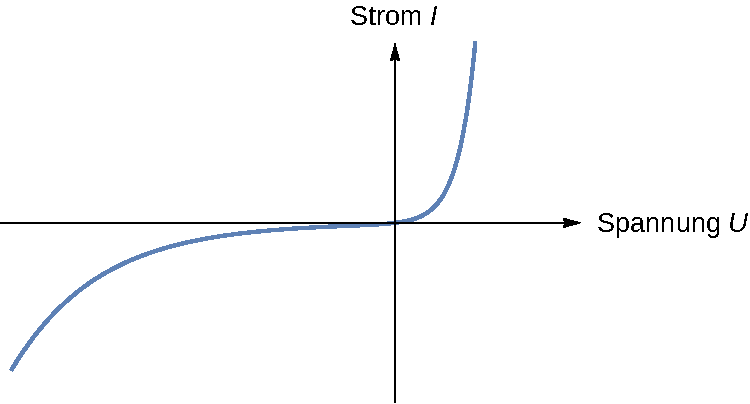
\includegraphics[width=0.6\textwidth]{../img/diode.pdf}
  \caption{Strom-Spannungskennlinie eins pn-Übergangs.
  Die Achsenskalierung ist nicht einheitlich.}
  \label{img:diode}
\end{center}
\end{figure}
Die asymmetrische Kennlinie kommt dadurch zustande,
dass der p-n-Übergang eine Durchlassrichtung (rechter Bereich der Abbildung) und eine Sperrrichtung
(linker Bereich) besitzt.
In Sperrrichtung fließt nur ein sehr kleiner Leckstrom, bis es bei hoher Spannung zum Durchbruch kommt.\\
Die Existenz einer Sperr- und einer Durchlassrichtung lässt sich anschaulich durch Vergrößerung
oder Verkleinerung der Raumladungszone erklären.
\autoref{img:pn} zeigt den Übergang zwischen einem p-dotierten und einem n-dotierten Halbleiter.
In der Kontaktzone wandern die Elektronen aus dem n-dotierten Material in das p-dotierte und hinterlassen
geladene Fehlstellen.
Die n-Seite ist dann positiv geladen, die p-Seite negativ.
Wird nun an den Halbleiter eine Spannung angelegt, so dass weitere Elektronen in die p-Schicht fließen,
vergrößert sich die Raumladungszone und es bildet sich ein Feld aus,
das der anliegenden Spannung entgegen wirkt.
Dieser Zustand herrscht in dem Halbleiter-Strahlungs-Detektor,
mit dem im dritten Versuchsteil Messungen durchgeführt werden.\\
Umgekehrt kann die Raumladungszone verkleinert werden,
wenn an die n-dotierte Schicht das negativere Potential angelegt wird.
Der p-n-Übergang wird dann leitend und sein Widerstand nimmt mit zunehmender Spannung ab.
\begin{figure}[H]
\begin{center}
  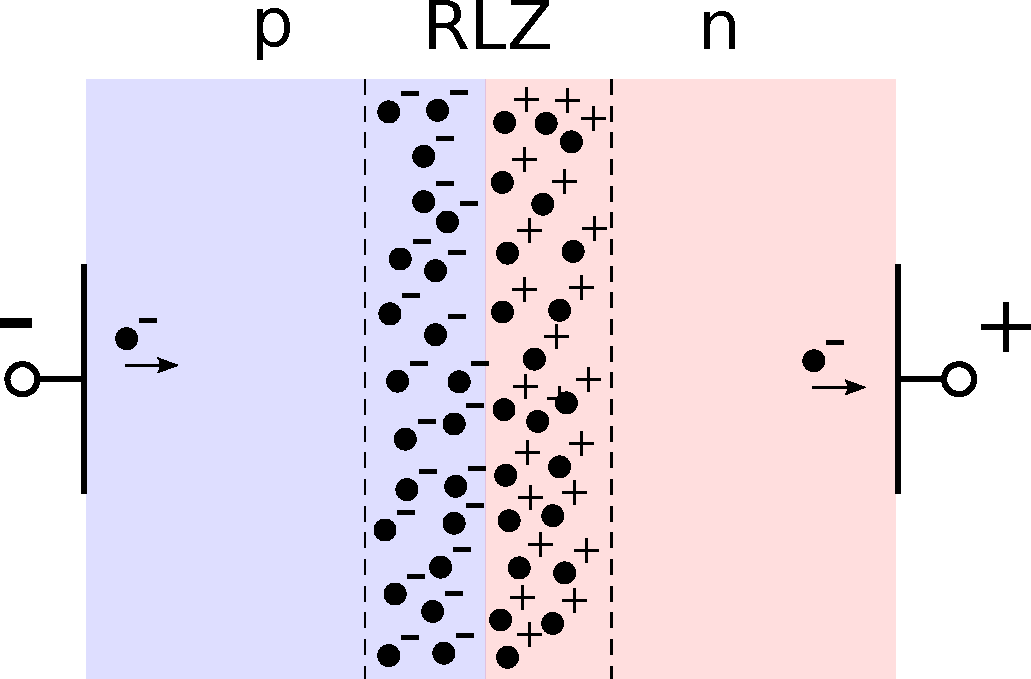
\includegraphics[width=0.6\textwidth]{../img/pn.pdf}
  \caption{Ausbildung einer Raumladungszone durch Verbindung von n- und p-dotierten Halbleitern
  und Vergrößerung der Raumladungszone durch Anlegen einer Spannung in Sperrrichtung.}
  \label{img:pn}
\end{center}
\end{figure}

\subsection{Ladungsträger in Halbleitern}

Die Bewegung der Ladungsträger in einem Halbleiter wird durch zwei Prozesse bestimmt:
\emph{Drift} und \emph{Diffision}.
Der Driftstrom $j_{\text{drift}}$ wird durch ein äußeres elektrisches Feld $E$ verursacht
und beträgt
\begin{equation}
\label{}
j_{\text{drift}}=\mu_{\text{n}} \cdot n \cdot E
\end{equation}
Die Mobilität der Elektronen (Verhältnis von Driftgeschwindigkeit zum angelegtem Feld) ist $\mu_{\text{n}}$,
die Ladungsträgerdichte wird als $n$ bezeichnet.
Eine räumliche Inhomogenität von $n$ führt zu einem Diffusionsstrom $j_{\text{diff}}$:
\begin{equation}
\label{}
j_{\text{diff}}=D_{\text{n}} \cdot \frac{\partial n}{\partial x}
\end{equation}
$D_{\text{n}}$ ist die materialspezifische Diffusionskonstante.\
Wegen Ladungserhaltung muss die Ladungsträgerdichte $n(t)$ die \emph{Kontinuitätsgleichung} erfüllen:
Die zeitliche Änderung der Elektronen im Leitungsband wird durch die Zahl der ins Valenzband
zurückfallenden Elektronen und die Divergenz des Stromes $j$ bestimmt:
\begin{equation}
\label{}
\frac{\partial n}{\partial t}= -\frac{n-n_0}{\tau_{\text{n}}}-\frac{\partial j}{\partial x}
\end{equation}
Die Ladungsträgerdichte im Gleichgewicht ist $n_0$, die mittlere Lebensdauer der Elektronen
im Leitungsband $\tau_{\text{n}}$.\\


DGLs lösen für Gaußkurve



TODO:Quelle: engl wiki, Haynes–Shockley experiment



\subsection{Lock-in-Verstärker}


Bilder mit Mathematica + Formeln

\subsection{++}
optisches Gitter\\
Energie(alpha)
